\vspace{1.5pc}
\section[Domain Penelitian]{Domain Penelitian}
\begin{spacing}{1.5}
	Domain dalam penelitian ini meliputi Samudra Hindia, Teluk Benggala, Laut Andaman, dan Selat Malaka dengan koordinat $0^\circ-24.6^\circ$ LU dan $76.96^\circ-104.96^\circ$ BT (lihat Gambar \ref{fig:domain}). Partikel mikroplastik disimulasikan dengan mengambil titik awal (\textit{starting point}) di beberapa lokasi perairan Aceh untuk melihat sebaran sampah plastik yang dibuang ke laut pada lokasi penelitian. 
	\begin{figure}[H]
		\centering
		\includegraphics[width=15cm]{contents/area_of_interest}
		\caption{Domain Penelitian}
		\label{fig:domain}
		\medspace
		\small
		Domain di plot dengan menggunakan data batimetri pada \href{https://www.naturalearthdata.com/}{https://www.naturalearthdata.com/} dengan skala resolusi 1:10m dari SRTM30+ dan dengan menggunakan library \href{https://scitools.org.uk/cartopy/docs/latest/getting_started/index.html#}{cartopy}, \href{https://matplotlib.org/}{matplotlib}, dan \href{https://seaborn.pydata.org/}{seaborn} dalam Python.
		
	\end{figure}
\end{spacing}
\section[Data Penelitian]{Data Penelitian}
\begin{spacing}{1.5}
\vspace{-1pc}
\subsection[Batimetri]{Batimetri}
	SRTM30+ adalah data digital model elevasi global (DEM) yang diperoleh dari radar SRTM (\textit{Instrument Shuttle Radar Topography}) untuk topografi darat dan ICESat (\textit{Ice, Cloud, and land Elevation SATellite}) untuk topografi es. Batimetri laut didasarkan dari model satelit graivitasi baru dimana rasio gravitasi-topografi dikalibrasi dengan menggunakan 298 juta suara yang diedit \shortcite{Becker2009}.
	\par Resolusi data SRTM30+ setiap spasial 1 arc-second pada bidang lintang dan bujur setara dengan 30 meter pada bidang ekuator (30 arc-second setara dengan 1 kilometer). Data batimetri dari Natural Earth Data menggunakan data SRTM30+ untuk menghasilkan peta dengan resolusi 10m (sangat detail), 50m (detail sedang), dan 110m (detail kasar). Peta Batimetri \ref{fig:domain} dalam penelitian ini menggunakan data resolusi 10m yang dapat didownload di \href{https://www.naturalearthdata.com/downloads/10m-physical-vectors/10m-bathymetry/}{https://www.naturalearthdata.com/}.
\subsection[Data NEMO]{Data NEMO}
	Penelitian ini menggunakan data output model NEMO (\href{https://www.nemo-ocean.eu/}{https://www.nemo-ocean.eu/}) untuk data analisis global arus tiga dimensi yang didownload dari website \href{https://resources.marine.copernicus.eu/products}{CMEMS} dari April 2021 - Maret 2022.  Dalam analisis kami, resolusi data output yang digunakan adalah dx = dy = 5 menit pada bidang horizontal dan 50-lapisan $(k \in [1,50])$ dengan ketebalan berbeda pada bidang vertikal:
	\begin{equation*}
		\begin{aligned}
			z_k = \{0.49, 1.54, 2.65, 3.82, 5.08, 6.44, 7.93, 9.57, 11.40, 13.47, 15.82, 18.50, \\
			21.60, 25.21, 29.44, 34.43, 40.34, 47.37, 55.76, 65.81, 77.85, 92.33, 109.73, 130.67, \\
			155.85, 186.12, 222.47, 266.04, 318.13, 380.21, 453.94, 541.089, 643.57, 763.33, \\
			902.34, 1062.44, 1245.29, 1452.25, 1684.28, 1941.89, 2225.08, 2533.33, 2865.70,  \\
			3220.82, 3597.03, 3992.48, 4405.22, 4833.29, 5274.78, 5727.92 \} (m). \\
		\end{aligned}
	\end{equation*}
	\par Model NEMO atau \textit{Nucleus for European Modeling of the Ocean} adalah model komputasi resolusi tinggi yang digunakan untuk kegiatan penelitian dan layanan peramalan dalam oseanografi dan klimatologi, yang dikembangkan secara berkelanjutan sejak tahun 2008 oleh konsorsium Eropa yang terdiri dari 5 institusi (CMCC | CNRS | Mercator Ocean | Met Office | NERC). Hal ini dimaksudkan untuk menjadi alat yang fleksibel untuk mempelajari fenomena fisik dan biogeokimia dalam sirkulasi laut, serta interaksinya dengan komponen sistem iklim Bumi, pada berbagai skala ruang dan waktu \cite{madec_gurvan_2022_6334656}.
\subsection[Data HYCOM]{Data HYCOM}
	Data HYCOM digunakan sebagai data perbandingan dalam penelitian ini. HYCOM (\textit{HYbrid Coordinate Ocean Model}) (\href{https://www.hycom.org}{https://www.hycom.org}) adalah salah satu model sirkulasi laut (OGCM) yang menggunakan model numerik tiga dimensi Navier-Stokes dengan input data batimetri dari GEBCO (\textit{General Bathymetric Chart of the Oceans}), data asimilasi hidrografi laut dari NCODA (\textit{Navy Coupled Ocean Data Assimilation}) dan komponen meteorologi dari NCEP (\textit{National Centers for Environmental Prediction}) ataupun NAVGEM (\textit{The NAVy Global Environmental Model}) berupa angin, kecepatan, fluks panas, tekanan permukaan laut, presipitasi, temperature, dan kelembapan \shortcite{JosephMetzger2013}. Koordinat vertikal dalam HYCOM adalah isopiknal di lautan terbuka yang terstratifikasi dan memiliki transisi yang mulus dan dinamis serta bergantung terhadap waktu pada medan daerah pesisir yang dangkal dan pada tingkat tekanan tetap di lapisan campuran permukaan atau lautan yang tidak terstratifikasi \shortcite{chassignet2017,Park2013}. 
	\par Data HYCOM yang digunakan adalah data analisis global arus tiga dimensi dengan resolusi spasial 5 menit untuk longitude dan 2.5 menit untuk latitude selama setahun (April 2021 - Maret 2022) dan dengan ketebalan bervariasi pada bidang vertikal, yaitu 40-lapisan $(k \in [1,40])$:
	\begin{equation*}
		\begin{aligned}
			z_k = \{0.0, 2.0, 4.0, 6.0, 8.0, 10.0, 12.0, 15.0, 20.0, 25.0, 30.0, 35.0, 40.0, 45.0, 50.0, \\
			60.0, 70.0,	80.0, 90.0, 100.0, 125.0, 150.0, 200.0, 250.0, 300.0, 350.0, 400.0, 500.0, 600.0,\\
			700.0, 800.0, 900.0, 1000.0, 1250.0, 1500.0, 2000.0, 2500.0, 3000.0, 4000.0, 5000.0\} (m). \\
		\end{aligned}
	\end{equation*}
\end{spacing}
\vspace{-1.5pc}
\section[Prosedur Penelitian]{Prosedur Penelitian}
\begin{spacing}{1.5}
	\begin{figure}[H]
		\centering
		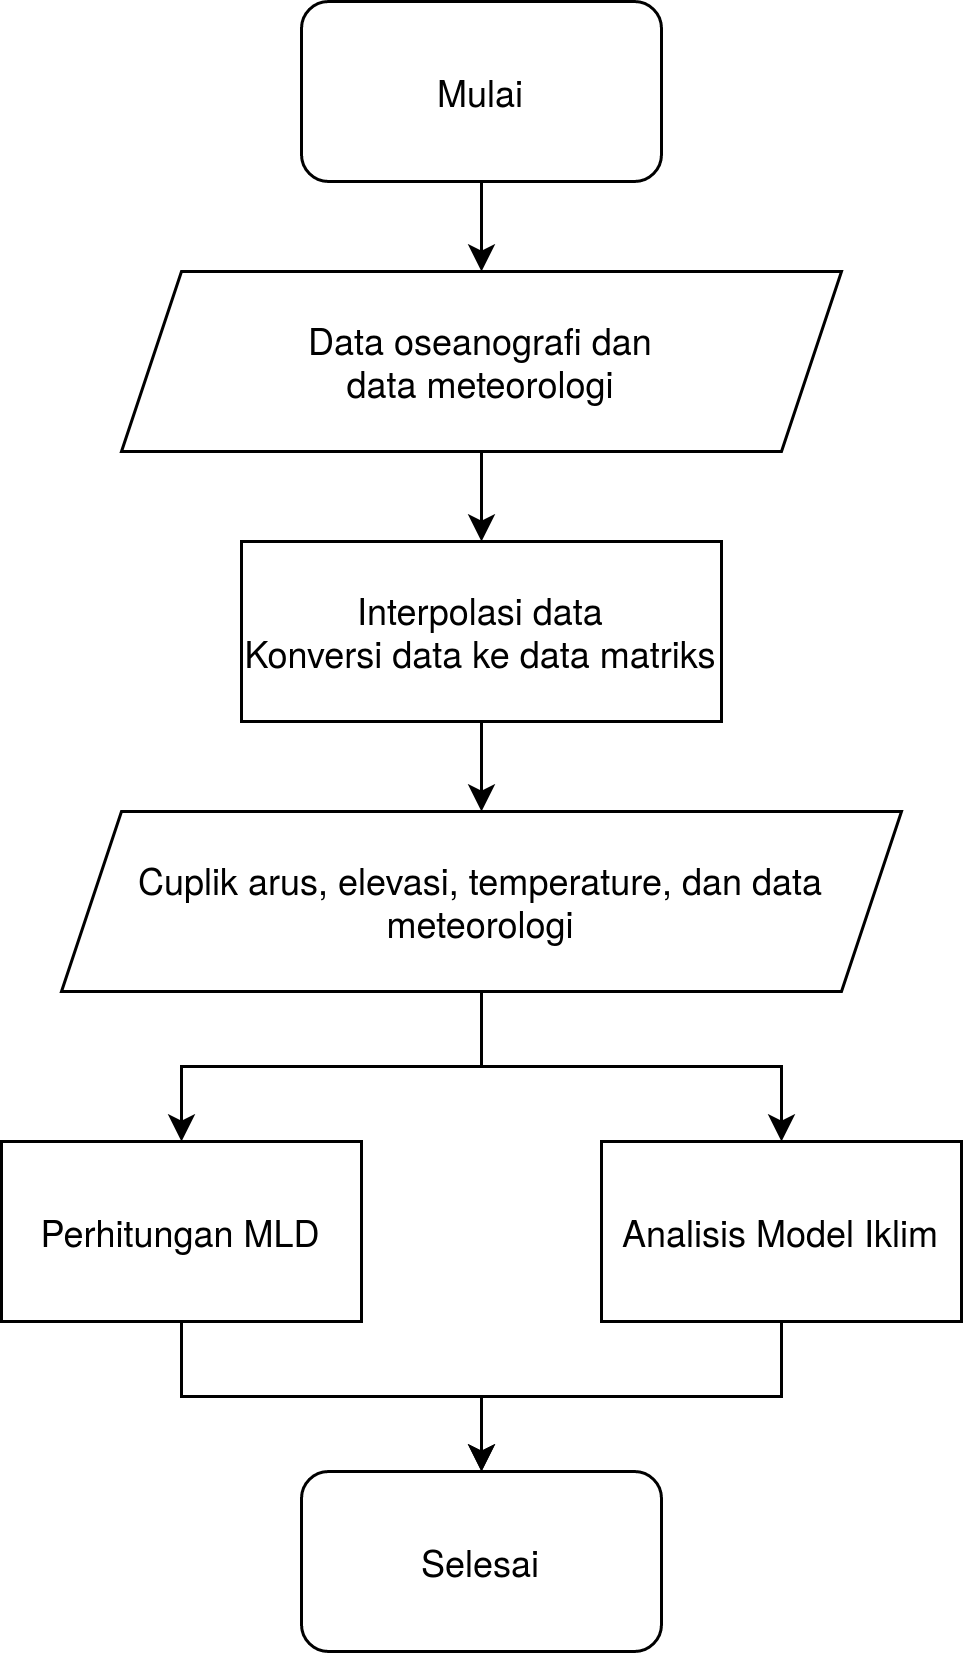
\includegraphics[width=15cm]{contents/flowchart.png}
		\caption{Diagram alir }
		\label{fig:flowchart}
	\end{figure}
	Prosedur penelitian mengikuti diagram alir pada Gambar \ref{fig:flowchart}. Pertama-tama akan dilakukan konfigurasi modul yang ada dalam Python untuk menentukan input langkah waktu simulasi yang digunakan, penentuan lokasi dan  jumlah partikel yang keluar, serta konfigurasi kernel dalam hal ini perlakuan partikel, perilaku, dan lama waktu penelitian. Selanjutnya data-data OGCM yang diperlukan didownload dari situs CMEMS, HYCOM, dan NCEP. Data-data yang telah didownload kemudian diinterpolasi agar sesuai dengan software Parcel yang digunakan dan disimpan dalam data \textit{field}. Setelah kernel didefinisikan dan dikonfigurasi, data \textit{field} kemudian diproses menggunakan algoritma Parcel dan dilakukan perulangan untuk waktu yang terintegrasi, dijalankan bersama dengan modul tambahan secara paralel serta memperbaharui kondisi partikel-partikel, dan menghasilkan output berupa NetCDF atau NumPy array. Langkah terakhir adalah proses analisis dan visualisasi hasil.
\end{spacing}